% SPDX-FileCopyrightText: 2023 SAP SE
%
% SPDX-License-Identifier: Apache-2.0
%
% This file is part of FEDEM - https://openfedem.org

%%%%%%%%%%%%%%%%%%%%%%%%%%%%%%%%%%%%%%%%%%%%%%%%%%%%%%%%%%%%%%%%%%%%%%%%%%%%%%%%
%
% FEDEM User Guide.
%
%%%%%%%%%%%%%%%%%%%%%%%%%%%%%%%%%%%%%%%%%%%%%%%%%%%%%%%%%%%%%%%%%%%%%%%%%%%%%%%%

\def\LinkFormatText#1{
  \medskip
  {\raggedright\tt#1}
  \medskip}

\def\LinkFormatTextNoSkip#1{{\raggedright\tt#1}}

\def\Variable#1{\textless#1\textgreater}


\Chapter{Beta feature documentation}{beta-feature-documentation}

Some new features in Fedem are still in a state of Beta testing.
These features are typically available through commands or options
entered in the description field of an entity's property panel.
This means to enter the special character {\tt\#} followed by a keyword and
possibly some values into the description field along with the user description,
like in the example shown below. See also
\refSection{property-editor}{Property Editor}.

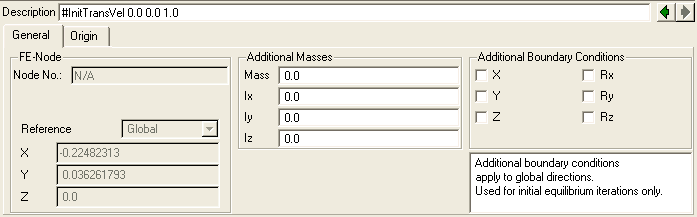
\includegraphics[width=0.9\textwidth]{Figures/F-PropertyPanel}

Due to the Beta nature of the features, they should be used with some care.
The present way of accessing these features through the options or commands in
the description field is subject to change, or no longer being supported,
in future releases. However, most of the features listed here will be supported
in a more "permanent" fashion in future releases.

Sections in this appendix address the following topics:

\begin{itemize}
\item\protect\hyperlink{joints-1}{Joints}
\item\protect\hyperlink{parts-1}{Parts}
\item\protect\hyperlink{beams-1}{Beams}
\item\protect\hyperlink{beam-properties-1}{Beam properties}
\item\protect\hyperlink{springs}{Springs}
\item\protect\hyperlink{frictions-1}{Frictions}
\item\protect\hyperlink{additional-masses}{Additional masses}
\item\protect\hyperlink{external-loads}{External loads}
\item\protect\hyperlink{sensors-1}{Sensors}
\item\protect\hyperlink{wave-functions}{Wave functions}
\item\protect\hyperlink{result-output-control-2}{Result output control}
\item\protect\hyperlink{undocumented-features}{Undocumented features}
\end{itemize}


%%%%%%%%%%%%%%%%%%%%%%%%%%%%%%%%%%%%%%%%%%%%%%%%%%%%%%%%%%%%%%%%%%%%%%%%%%%%%%%%
\Section{Joints}{joints-1}

\SubSection{Universal Joint}{universal-joint}

The universal joint is obtained from the Ball Joint when the command

\LinkFormatText{\#UniversalJoint}

\noindent
is entered in the description field of the selected Ball Joint.
The initial orientation of the joint cross is assumed to be the $Y$- and
$Z$-axis of the Ball Joint master triad. The $Z$-axis of the cross is connected
to the master part whereas the $Y$-axis is connected to the slave part.
The user must thus reorient the master triad appropriately for the desired joint
configuration.
Attention must also be paid to the selection of master versus slave part.


\SubSection{Constant Velocity Joint}{constant-velocity-joint}

A constant velocity joint is obtained from a Ball Joint when the command

\LinkFormatText{\#CVJoint [\#RZ \Variable{float}] [\#RY \Variable{float}]}

\noindent
is entered in the description field of the selected Ball Joint.

The $X$-axis of the master triad should be oriented along the rotation axis of
the master shaft (part). The direction of the slave shaft rotation axis,
the $X$-axis, is determined by one, or both, of the optional commands

\LinkFormatText{\#RZ \Variable{float} \#RY \Variable{float}}

\noindent
{\tt\#RZ} gives direction of slave $X$-axis relative to master $X$-axis by a
rotation about the $Z$-axis of the master triad. {\tt\#RY} obtains the $X$-axis
from the master $X$-axis by a rotation about the $Y$-axis of the master triad.
Care should be exercised when applying both rotations since the angles are
{\sl Euler-Z-Y} rotations. It is recommended that the master triad is oriented
such that one only needs to use one of the command {\tt\#RZ} and {\tt\#RY}.

\Note{The universal joint and constant velocity joint have both only two
  independent joint DOFs (the Y- and Z-rotations). Specifying a spring
  stiffness and/or damping for the third DOF (X-rotation) for these joint
  types is therefore meaningless, although that is possible in the
  Property Editor panel. Any spring/damper properties specified on this
  DOF will be silently ignored. The same is true for initial conditions.}

\clearpage


\SubSection{Rigid Joint}{rigid-joint-1}

The DOFs of the Rigid Joint can be released individually by entering one
or more of the commands

\LinkFormatText{\#FreeX \#FreeY \#FreeZ \#FreeRX \#FreeRY \#FreeRZ}

\noindent
in the description field of the selected Rigid Joint. The rotational
parameterization is rotation axis components. All DOFs are referred to
master triad coordinate system.


\SubSection{Axial Joint}{axial-joint}

An Axial Joint is obtained from the Free Joint when the command

\LinkFormatText{\#Axial}

\noindent
is entered in the description field of the selected Free Joint.
This is a single-DOF joint that works like an Axial Spring and/or Damper,
except that the length between the two triads here is used as a joint DOF.
The {\sl Tx} tab of the joint property panel (see \refSection{joint-properties}
{Joint properties}) is used to control the behavior of the length DOF.
All the other DOF tabs of the property panel are not used when {\tt\#Axial}
is specified.

The advantage of using an Axial Joint opposed to a combined Axial Spring
and Damper is that you are able to prescribe the length between the two
triads directly, without the need for stiff springs and associated
damping, which might render the model numerically unstable. It also
reduces the total number of DOFs in the mechanism compared with an Axial
Spring/Damper (reduced by 5 for each Axial Joint). More details on the
formulation of the Axial Joint may be found in the
\FedemTGuide{Section 6.2.7, "Axial Joint"}.


\SubSection{Free Joint}{free-joint-1}

By default, the translational- and rotational DOFs are coupled in a Free Joint.
It is possible to remove this coupling by entering the following description
field command

\LinkFormatText{\#noRotTransCoupling}

\noindent
The Free Joint will then not transfer any bending moments due to eccentric
master and slave triad locations.
It will therefore behave more like a Ball Joint, if the translational DOFs
are fixed or have been assigned a hight stiffness.

An alternative Free Joint formulation is available through the
specification of the following description field command

\LinkFormatText{\#GlobalSpring}

\noindent
The default master-slave joint formulation is then not used (which for
the Free Joint only is a transformation of the free DOFs from the slave
Triad to the joint variables, and no constraining). With the alternative
formulation the added spring (and damper) properties are applied
directly in the global coordinate directions between the two triads
instead, and no change in free variables is performed. There are no
eccentricity contributions either when the force between the two triads
is not attacking along their common axis. Consequently, this free joint
is somewhat equivalent to a BUSH element on the system level (see the
\FedemTGuide{Section E.10, "BUSH"}).

It is also possible to specify coupling stiffnesses in a free joint
when using the {\tt\#GlobalSpring} command.
This is done by appending the following to the description:

\LinkFormatText{\#K\Variable{i}\Variable{j} \Variable{kij}}

\noindent
where {\tt\Variable{kij}} is the constant coupling stiffness between
the local DOFs {\tt\Variable{i}} and {\tt\Variable{j}} in the free joint.
It is not possible to specify non-constant coupling stiffness values.


\SubSection{Prismatic Joint and Cylindric Joint}
           {prismatic-joint-and-cylindric-joint}

Both Prismatic and Cylindric Joint can take the command

\LinkFormatText{\#Extended}

\noindent
in the description field. Entering this command allows the follower to
travel beyond the first and last triad of the track. When the follower
is past the beginning of the track, the first two triads receive the
contact force in a statically consistent manner. When the follower is
past the last triad the last two triads receive the contact force.

By default, the contact force is interpolated linearly between the two
triads on both side of the follower, based on their relative location.
However, a cubic interpolation using the four closest master triads at
any time can be used instead, by specifying the description field command

\LinkFormatText{\#Cubic}

The default rotational parameterization of the Cylindric Joint is
{\sl Euler-Z-Y-X rotations}, but this can be changed to components of the
rotation axis vector by entering the command

\LinkFormatText{\#RotAxisParam}

\noindent
in the description field of the selected Cylindric Joint. This command
can also be applied to the Cam Joint when the alternative master-slave
based formulation is used (see \refSection{cam-joint-1}{Cam Joint} below).


\SubSection{Cam Joint}{cam-joint-1}

The default cam formulation uses non-linear springs to model contact
between the follower (slave triad) and the master triads along the cam curve.
This formulation has independent DOFs at the follower and all master triads,
and is able to handle large separation between cam and follower.

An alternative formulation, in which the motion of the follower is
expressed in a curvilinear coordinate system surrounding the cam surface
and the slave triad is treated more like a true slave of the master triads,
is obtained by entering the following command in the description field:

\LinkFormatText{\#MasterSlaveCam}

\noindent
With this formulation one can also enter one, or both, of the commands:

\LinkFormatText{\#FixX \#FixY}

\noindent
The joint DOFs in these directions are then eliminated (along with the
joint springs and dampers), and the follower is restricted to follow the
cam in that direction. Using these options can give a numerically more
stable formulation when no separation between the cam and follower is
expected (or possible). The master-slave cam formulation is only able to
handle small separation (relative to the cam-segment radius) between
follower and cam surface. A cam surface with corners can also cause
problems with this alternative formulation.


%%%%%%%%%%%%%%%%%%%%%%%%%%%%%%%%%%%%%%%%%%%%%%%%%%%%%%%%%%%%%%%%%%%%%%%%%%%%%%%%
\Section{Parts}{parts-1}

\SubSection{Geometric stiffness}{geometric-stiffness}

The {\sl Geometric stiffness contribution} toggle in the
\protect\hyperlink{integration-tab}{\sl Integration tab} of the Dynamics Solver
dialog box (see
\refSection{dynamics-solver-advanced-mode}{Dynamics Solver (Advanced Mode)})
applies normally to all flexible parts in the model during the dynamics
simulation. It is possible to override this setting for a specific part
using the following description field commands:

\medskip
\LinkFormatTextNoSkip{\#DynStressStiffening}
\tabto{45mm} -- Enables geometric stiffness for this part

\LinkFormatTextNoSkip{\#NoDynStressStiffening}
\tabto{45mm} -- Disables geometric stiffness for this part
\medskip

\noindent
The commands affect the dynamics simulation only. They have no effect during the
initial equilibrium and eigenmode analyses. They also have no effect for
generic parts with automatic stiffness calculation toggled on.


\SubSection{Component modes}{component-modes}

The number of {\sl Component modes} that is entered in the Property Editor panel
for a selected part, defines how many component mode shapes that should be
computed during the reduction of that part, see
\refSubSection{reduction-options-tab}{Reduction Options tab}{part-properties}.
Thus, whenever you change this number, the part might need to be reduced again.
The default is to use all the computed component mode shapes as DOFs for the
part during the dynamics simulation. However, it is possible to use only a
subset of the computed modes, by specifying the following description field
commands for the part:

\medskip
\LinkFormatTextNoSkip{\#InclModes\Variable{m1}\Variable{m2}...}
\tabto{45mm} -- Use only these component modes

\LinkFormatTextNoSkip{\#ExclModes\Variable{m1}\Variable{m2}...}
\tabto{45mm} -- Use all but these component modes
\medskip

The structural damping parameters entered in the Property Editor panel
for a part, see \refSubSection{part-tab}{Part tab}{part-properties},
are by default applied to the whole stiffness- and mass matrix of the part.
However, it is possible to specify individual Rayleigh damping factors for each
of the component modes through the following description field commands:

\medskip
\LinkFormatTextNoSkip{\#Alpha1\Variable{c1}\Variable{c2}...}
\tabto{45mm} -- Mass-proportional damping factors\newline
\tabto{48mm} for the component modes

\LinkFormatTextNoSkip{\#Alpha2\Variable{c1}\Variable{c2}...}
\tabto{45mm} -- Stiffness-proportional damping factors\newline
\tabto{48mm} for the component modes
\vskip\parskip

\noindent
Thus, {\tt\Variable{c1}} is the damping factor applied to the first
component mode used, {\tt\Variable{c2}} is the factor for the second
mode, etc. If you specify fewer such individual damping factors than the number
of component modes being used, the last value entered is used for all the
remaining modes.


\SubSection{Initial velocities}{initial-velocities}

A uniform initial translational velocity that applies to the entire
model may be specified in the Model Preferences dialog box (see
\refSection{model-preferences}{Model preferences}). An
alternative is to specify initial conditions to individual parts,
through the following description field command:

\LinkFormatText{\#InitTransVel \Variable{ux} \Variable{uz}}

\noindent
The values {\tt\Variable{ux}, \Variable{uy}} and
{\tt\Variable{uz}} are then applied to all triads attached to that
part, including the automatically generated center of gravity triad for generic
parts. This is overridden by any non-zero initial velocity specified in the
Triad property panel though.

For generic parts, the center of gravity triad can also be assigned an initial
rotational velocity through a similar description field command

\LinkFormatText{\#InitRotVel \Variable{rx} \Variable{ry} \Variable{rz}}


\SubSection{Stress recovery on element groups during dynamics simulation}
           {stress-recovery-on-element-groups-during-dynamics-simulation}

Doing stress recovery on entire FE parts during the dynamics simulation,
as described in
\refSection{stress-and-strain-recovery-during-time-integration}
{Stress and strain recovery during time integration},
is time and memory consuming. Often it is sufficient to limit this
calculation to a sub-set of the FE part, which will be more efficient.

Use one of the following description-field commands for stress recovery
during the dynamics simulation on specified element groups in a FE part:

\medskip
\LinkFormatTextNoSkip{\#recover-stress gid}

\LinkFormatTextNoSkip{\#recover-stress \Variable{gid1,gid2,...}}

\LinkFormatTextNoSkip{\#recover-stress \Variable{PMAT id1,PTHICK id2,...}}
\medskip

\noindent
The first two commands will calculate internal displacements and von Mises
stresses for all elements in one or several element groups ({\tt gid} and
{\tt gid\Variable{i}} are user IDs of the element groups to do recovery on).
The third command can be used when recovery on implicit element groups is
wanted, defined via the specified element properties (see
\refSection{element-groups}{Element groups} for more information
on implicit element groups).
Here, {\tt id\Variable{i}} represents the IDs of the element group property.


%%%%%%%%%%%%%%%%%%%%%%%%%%%%%%%%%%%%%%%%%%%%%%%%%%%%%%%%%%%%%%%%%%%%%%%%%%%%%%%%
\Section{Beams}{beams-1}

\SubSection{Structural damping}{structural-damping}

The stiffness-proportional damping coefficient ($\alpha$\textsubscript{2}) for
a Beam element may be defined via a Function, through the command

\LinkFormatText{\#StructDmpEngine \Variable{id}}

\noindent
where {\tt\Variable{id}} is the base ID of the Function defining the damping
factor. The same command can also be applied on FE and Generic Parts.

\Note{The base ID of a mechanism object is normally not visible in the Model
  Manager panel. To see them, you have to launch Fedem in debug mode
  (using command-line option {\tt-debug}). Then the base ID appears in curly
  braces \{\} in the Objects list. You can also use the Object
  Browser dialog box, see \refSection{object-browser}{Object Browser}.}


\SubSection{Time-dependent stiffness scaling}
           {time-dependent-stiffness-scaling}

The stiffness matrix of a Beam element can be adjusted using a time- or
state-dependent scale function through the description field command:

\LinkFormatText{\#StiffScaleEngine \Variable{id}}

\noindent
The {\tt\Variable{id}} is the base ID of the desired scaling function.

The same command can also be applied on Generic Parts. However, it is not
recommended to use it on FE Parts if you also are going to perform stress
recovery on that part. This is because the displacement recovery operator,
calculated during the FE Part reduction, does not account for the stiffness
scaling factor such that the calculation of internal deformation and stresses
will be incorrect.


\SubSection{Beam diagram curve domain adjustment}
           {beam-diagram-curve-domain-adjustment}

When plotting results along beams
(see \refSection{beam-diagrams}{Beam diagrams}), all beam elements
along a string from a selected start Triad or Beam are considered, until the
end of the beam string or a joint between several beam elements is detected.
To create a beam diagram that stops at any beam element before the end
or a joint is reached, the following description field command is entered
for the desired end element:

\LinkFormatText{\#Stop}

\noindent
A beam diagram curve can normally be started from a ``natural'' end of a beam
string as described above. However, it is possible to start a curve from any
intermediate beam element, if the following command is entered
for the desired element:

\LinkFormatText{\#Start}


%%%%%%%%%%%%%%%%%%%%%%%%%%%%%%%%%%%%%%%%%%%%%%%%%%%%%%%%%%%%%%%%%%%%%%%%%%%%%%%%
\Section{Beam properties}{beam-properties-1}

For beam cross section objects with Hydrodynamics enabled, one may specify a
{\sl slamming} load coefficient through the following command:

\LinkFormatText{\#Cs \Variable{Cs} \Variable{Tcs}}

\noindent
where {\tt\Variable{Cs}} is the actual slamming coefficient and
{\tt\Variable{Tcs}} is the duration time of the slamming load.


%%%%%%%%%%%%%%%%%%%%%%%%%%%%%%%%%%%%%%%%%%%%%%%%%%%%%%%%%%%%%%%%%%%%%%%%%%%%%%%%
\Section{Springs}{springs}

\SubSection{Sign-dependent stiffness scaling}
           {sign-dependent-stiffness-scaling}

Spring stiffness for both axial and joint springs can be adjusted using
scale functions. Different adjustment for positive and negative deflection of
a spring is often desirable when adjusting the stiffness of, for instance,
hydraulic cylinders. To achieve this, use the description field commands:

\medskip
\LinkFormatTextNoSkip{\#PosStiffScaleEngine \Variable{id}}

\LinkFormatTextNoSkip{\#NegStiffScaleEngine \Variable{id}}
\medskip

\noindent
where the {\tt\Variable{id}} is the function's base ID.
These commands set the scale function only for the respective deflection state.
If used, they will override the scale function selected through the Spring
property panel, if any.

\Tip{You can access the description field of a joint spring by double-clicking
  the desired spring entry in the Topology view of the actual joint.}


\SubSection{Plastic springs}{plastic-springs}

For springs using a nonlinear force-deflection curve as stiffness
characteristics, the following command may be used to define a
cyclic-plastic behavior:

\LinkFormatText{\#Cyclic [\Variable{flag}]}

\noindent
where {\tt\Variable{flag}} is an optional integer value to specify how
the spring behaves during unloading.

\begin{itemize}
\item{\tt flag} = 1 : Unloading occurs with initial tangent stiffness (for
  positive deflections only). This is the default if not flag value is given.
\item{\tt flag} = 2 : Reserved for future used.
\item{\tt flag} = 3 : Unloading occurs using the secant stiffness,
  for both positive and negative deflections.
\end{itemize}


\SubSection{Spring failure}{spring-failure}

When a joint spring has been assigned failure criteria through an
Advanced spring characteristics object (see
\refSection{advanced-spring-characteristics}{Advanced spring characteristics}),
it is often desirable when that spring fails (i.e., the spring force and
stiffness both drop to zero for any deflection level), that all the other
springs in the same joint having failure criteria assigned should fail in the
same instant such that the entire joint is decoupled.
This is accomplished by specifying the following description field command for
the Advanced spring characteristics object that the spring refers to:

\LinkFormatText{\#FailAll}


\SubSection{Stiffness proportional damping}
           {stiffness-proportional-damping}

Axial springs can be assigned a stiffness-proportional damping
coefficient by specifying the following description field command:

\LinkFormatText{\#Rayleigh \Variable{alpha2}}

\noindent
where {\tt\Variable{alpha2}} is the stiffness-proportional damping coefficient.


\SubSection{Pulley element}{pulley-element}

An axial spring can be assigned one (or more, up to 8) extra triads to simulate
a pulley system. This is done by specifying the following description field
command for the Axial spring object:

\LinkFormatText{\#addTriads \Variable{id1} \Variable{id2} ...}

\noindent
where {\tt\Variable{id1} \Variable{id2} ...} are base IDs of the extra triads.


%%%%%%%%%%%%%%%%%%%%%%%%%%%%%%%%%%%%%%%%%%%%%%%%%%%%%%%%%%%%%%%%%%%%%%%%%%%%%%%%
\Section{Frictions}{frictions-1}

An alternative friction formulation is available by specifying the
following command in the description field of a friction object:

\LinkFormatText{\#Kstick \Variable{k}}

\noindent
where {\tt\Variable{k}} is the stiffness used to enforce no movement in
the friction DOF when in stick condition.
This formulation is based on the use of a spring with varying yield criterion
(see \refSection{advanced-spring-characteristics}
{Advanced spring characteristics}). That is, the Max Yield Force is
taken as the maximum occurring friction force before the friction DOF
is slipping (see \FedemTGuide{Section 6.5.4, "Total friction"}).
The equivalent load for the friction calculation may be specified
explicitly instead of relying on the formulas defined in the
\FedemTGuide{Section 6.5, "Joint friction"}.
This is done using the description field command

\LinkFormatText{\#FrictionForceEngine \Variable{id}}

\noindent
where {\tt\Variable{id}} is the base ID of a Function that defines
the equivalent load.


%%%%%%%%%%%%%%%%%%%%%%%%%%%%%%%%%%%%%%%%%%%%%%%%%%%%%%%%%%%%%%%%%%%%%%
\Section{Additional masses}{additional-masses}

The additional masses are scaled using a Function when the command

\LinkFormatText{\#MassScaleEngine \Variable{id}}

\noindent
is entered in the description field for the selected Triad.
The {\tt\Variable{id}} is the function's base ID.
The additional rotational inertias for the selected triad are also scaled using
the same function.

The additional masses may be applied in a specified local triad direction only,
by specifying one of the following commands in the Triad description field
(the commands only affects the translational mass):

\LinkFormatText{\#MassDir \Variable{cx} \Variable{cy} \Variable{cz}}

\LinkFormatText{\#MassX \#MassY \#MassZ}

\noindent
where {\tt\Variable{cx}}, {\tt\Variable{cy}} and {\tt\Variable{cz}} defines the
local triad direction the additional mass should be applied in.
{\tt\#MassX} is equivalent to {\tt\#MassDir 1 0 0}, {\tt\#MassY} is equivalent
to {\tt\#MassDir 0 1 0} and {\tt\#MassZ} is equivalent to {\tt\#MassDir 0 0 1}.

\clearpage
An additional mass is regarded as a {\sl virtual added mass} when

\LinkFormatText{\#AddedMass \Variable{mx} \Variable{my} \Variable{mz}}

\noindent
is entered in the description field of the Triad description field.
The additional mass then contributes to the mass matrix and inertia forces only,
and not to the gravitational force vector. The added mass terms then equal
\{{\tt\Variable{M}*\Variable{mx}, \Variable{M}*\Variable{my},
\Variable{M}*\Variable{mz}}\} in the local triad directions,
where {\tt\Variable{M}} is the value specified in the {\sl Mass} field.


%%%%%%%%%%%%%%%%%%%%%%%%%%%%%%%%%%%%%%%%%%%%%%%%%%%%%%%%%%%%%%%%%%%%%%%%%%%%%%%%
\Section{External loads}{external-loads}

Time- or state-dependent external loads can be updated based on the previous
time instead of the current time, by specifying the description field command

\LinkFormatText{\#PrevStep}

External loads in triads DOFs are applied in the defined system directions
of the Triad, i.e., the same axis system boundary conditions are applied in,
see \refSection{triad-properties}{Triad properties}.
This is normally equivalent to the global axis system. It is, however,
also possible to let the loads act in the local with-rotated axis system
independent of the chosen System directions, by specifying the command

\LinkFormatText{\#LocalAxes}

\noindent
in the description field of the load object. This is equivalent to the
default behavior in Fedem R7.3.0 and earlier releases.

\Tip{You can access the description field of a Triad DOF load by double-clicking
  the desired load entry in the Topology view of the actual triad.}


%%%%%%%%%%%%%%%%%%%%%%%%%%%%%%%%%%%%%%%%%%%%%%%%%%%%%%%%%%%%%%%%%%%%%%%%%%%%%%%%
\Section{Sensors}{sensors-1}

Sensors on triads can measure rotations in terms of Rodriguez rotations
by entering the command

\LinkFormatText{\#Rodrig}

\noindent
in the description field for the selected Sensor. The angular quantities
measured by this sensor are then the component of rotation vector, as defined in
the \FedemTGuide{Section 2.3.3, "Rodriguez parameterization"}.
The default is to measure {\sl Euler-Z-Y-X} angles.

General functions using the default function argument, {\sl Time}, can instead
use the number of nonlinear iterations spent on the previous time step as
argument, by specifying the following description field command:

\LinkFormatText{\#NumIt}


%%%%%%%%%%%%%%%%%%%%%%%%%%%%%%%%%%%%%%%%%%%%%%%%%%%%%%%%%%%%%%%%%%%%%%%%%%%%%%%%
\Section{Wave functions}{wave-functions}

\SubSection{Regular wave functions}{regular-wave-functions}

Higher-order regular wave functions are defined from a regular Sine wave
function through the following description field commands:

\medskip
\LinkFormatTextNoSkip{\#Stokes5}
\tabto{18mm} -- $5^{th}$ order Stokes wave function

\LinkFormatTextNoSkip{\#Stream}
\tabto{18mm} -- Nonlinear streamline wave function
\medskip


\SubSection{Irregular wave functions}{irregular-wave-functions}

The frequency range of wave functions of type JONSWAP sea wave spectrum is
calculated automatically or through user-defined period cut-off values specified
in the property panel of the wave function. However, to specify the frequency
interval explicitly, the following description field command can be used:

\LinkFormatText{\#OmegaRange \Variable{w0} \Variable{w1}}

\noindent
where \Variable{w0} and \Variable{w1} are, respectively,
the lowest and the highest frequency in the wave spectrum.


\SubSection{Embedded streamline functions}
           {embedded-streamline-functions}

It is possible to blend in one (or several) nonlinear streamline wave
function(s) into a irregular wave function defined from a JONSWAP spectrum.
This is done through the following description field command:

\LinkFormatText{\#EmbeddedStream \Variable{r1} \Variable{r2}
                \Variable{t0} \Variable{Tp} \Variable{H}}

\begin{itemize}
\item{\tt r1}, {\tt r2} :
  Blending parameters (see equation below), $0<{\tt r1}<{\tt r2}<1$
\item{\tt t0} :
  The time at which the embedded streamline wave should occur
\item{\tt Tp} :
  Period of the embedded streamline wave function
\item{\tt H} :
  Wave hight of the embedded streamline wave function
\end{itemize}

\noindent
The resulting wave elevation function is then established as follows:
$$
\eta(x,t) = \frac{1}{2}\left(\eta_{JS}(x,t)(1-w(t))+\eta_{SL}(x,t)(1+w(t))\right)
$$
where $\eta_{JS}(x,t)$ and $\eta_{SL}(x,t)$ are the wave elevations of the
background JONSWAP irregular wave and the streamline wave, respectively,
and $w(t)$ is a weighting (blending) function defined as:
$$
w(t) = \cos\left(\pi\frac{|t-t_0|-r_1 T_p}{(r_2-r_1)T_p}\right)
\;,\quad |t-t_0| \;\in\; [r_1T_p,r_2 Tp])
$$
whereas $w(t)=1$ for $|t-t_0|<r_1T_p$ and $|t-t_0|>r_2T_p$.


%%%%%%%%%%%%%%%%%%%%%%%%%%%%%%%%%%%%%%%%%%%%%%%%%%%%%%%%%%%%%%%%%%%%%%%%%%%%%%%%
\Section{Result output control}{result-output-control-2}

Simulating large models over long time series will generate a lot of
results data. Users may then be interested in the results for only a few
objects of a certain type, in order to reduce the size of the result
database files. To facilitate such output selection, the options
{\tt-allPrimaryVars-} and {\tt-allSecondaryVars-} may be specified
as additional solver options for the Dynamics Solver
\refSection{additional-solver-options}{Additional solvercoptions} to switch off
all output of primary and secondary solution variables, respectively.

The following two description field commands are then provided to enable
output for specific objects:

\LinkFormatText{\#savePos}

\noindent
This command enables saving of the position matrix for Triads, Parts and
Beam objects in the model when {\tt-allPrimaryVars-} is used.
It has no effect for other object types.

\LinkFormatText{\#savevar \Variable{f1}  \Variable{f2} ... \Variable{fn}}

\noindent
where the {\tt\Variable{f\sl i}} flags have the value 0 or 1 indicating whether
a certain variable is to be saved for that object or not.
This command is effective when the option {\tt-allSecondaryVars-} is used.
The number of flags in the {\tt\#saveVar} command varies depending on the type
of object it is used for. The flags have the interpretation as shown in the
following for the different object types.


\SubSection{Triads}{triads-1}

\LinkFormatText{\#savevar \Variable{f1} \Variable{f2} \Variable{f3}
                          \Variable{f4} \Variable{f5} \Variable{f6}}

\begin{itemize}
\item{\tt f1} : Global velocity
\item{\tt f2} : Global acceleration
\item{\tt f3} : Global forces
\item{\tt f4} : Local velocity
\item{\tt f5} : Local acceleration
\item{\tt f6} : Local forces
\item{\tt f7} : Global deformations
\end{itemize}


\SubSection{Parts}{parts-2}

\LinkFormatText{\#savevar \Variable{f1} \Variable{f2} \Variable{f3}}

\begin{itemize}
\item{\tt f1} : Center of gravity
\item{\tt f2} : Generalized DOF components (displacement, velocity acceleration)
\item{\tt f3} : Energies
\end{itemize}


\SubSection{Beams}{beams-2}

\LinkFormatText{\#savevar \Variable{f1} \Variable{f2} \Variable{f3}}

\begin{itemize}
\item{\tt f1} : Center of gravity
\item{\tt f2} : End sectional forces
\item{\tt f3} : Energies
\end{itemize}

\clearpage


\SubSection{Joints}{joints-2}

For joints, the {\tt\#savevar} flags are specified in groups of five,
where each group is associated with the corresponding joint DOF.

\LinkFormatText{\#savevar
                \Variable{f1}$_1$ \Variable{f2}$_1$ \Variable{f3}$_1$
                \Variable{f4}$_1$ \Variable{f5}$_1$ \\
  \hspace*{17mm}\Variable{f1}$_2$ \Variable{f2}$_2$ \Variable{f3}$_2$
                \Variable{f4}$_2$ \Variable{f5}$_2$ ... \\
  \hspace*{17mm}\Variable{f1}$_n$ \Variable{f2}$_n$ \Variable{f3}$_n$
                \Variable{f4}$_n$ \Variable{f5}$_n$}

\begin{itemize}
\item{\tt f1$_i$} : Deflection in joint DOF $i$
\item{\tt f2$_i$} : Velocity in joint DOF $i$
\item{\tt f3$_i$} : Acceleration in joint DOF $i$
\item{\tt f4$_i$} : Friction/reaction force in joint DOF $i$
\item{\tt f5$_i$} : Friction energy in joint DOF $i$
\end{itemize}

\noindent
The {\tt\Variable{f4}$_i$} flag toggles the output of friction force if the
joint DOF $i$ is either Free or Spring--Damper constrained, and the reaction
force if the joint DOF is either Fixed or Prescribed.
To toggle output of the spring and/or damper forces in a spring-damper
constrained joint DOF, you have to specify appropriate
{\tt\#savevar} flags on the joint spring and damper objects as given in
\refSection{springs-1}{Springs} and \refSection{dampers}{Dampers}, respectively.
To access the description fields of these objects, right-click the desired joint
spring/damper object in the {\sl Topology} view and choose \textbf{Select},
see \refSection{id-and-topology-panel}{ID and Topology panel}.


\SubSection{Springs}{springs-1}

\LinkFormatText{\#savevar
                \Variable{f1} \Variable{f2} \Variable{f3}
                \Variable{f4} \Variable{f5}}

\begin{itemize}
\item{\tt f1} : Spring stiffness
\item{\tt f2} : Spring length
\item{\tt f3} : Spring deflection
\item{\tt f4} : Spring force
\item{\tt f5} : Energies
\end{itemize}

\clearpage


\SubSection{Dampers}{dampers}

\LinkFormatText{\#savevar
                \Variable{f1} \Variable{f2} \Variable{f3}
                \Variable{f4} \Variable{f5}}

\begin{itemize}
\item{\tt f1} : Damping coefficient
\item{\tt f2} : Damper length
\item{\tt f3} : Damper velocity
\item{\tt f4} : Damping force
\item{\tt f5} : Energies
\end{itemize}


\SubSection{Loads (Force and Torque)}{loads-force-and-torque}

\LinkFormatText{\#savevar \Variable{f1} \Variable{f2} \Variable{f3}}

\begin{itemize}
\item{\tt f1} : Global force/torque vector
\item{\tt f2} : Signed force/torque amplitude
\item{\tt f3} : Energies
\end{itemize}


\SubSection{Mechanism}{mechanism}

\LinkFormatText{\#savevar \Variable{f1} \Variable{f2} \Variable{f3}}

\begin{itemize}
\item{\tt f1} : Center of gravity
\item{\tt f2} : Energies
\item{\tt f3} : Algorithm parameters
\end{itemize}

\Note{The {\tt\#savevar} command of the Mechanism object is entered in the
  Model description field of the Model Preferences dialog box, see
  \refSection{model-preferences}{Model preferences}.}


%%%%%%%%%%%%%%%%%%%%%%%%%%%%%%%%%%%%%%%%%%%%%%%%%%%%%%%%%%%%%%%%%%%%%%%%%%%%%%%%
\Section{Undocumented features}{undocumented-features}

In addition to the description field commands discussed in the above sections,
there also exists another set of commands without any further documentation.
They are used for features that are still under testing, or as a back-door for
some special-purpose features. For the sake of completeness,
these commands are listed in the table below.

\Warning{Do not use any of these commands unless you know what you are doing.
  If you encounter a Fedem model file where one or more of them are being used,
  please consult the Fedem support team before using that file.}

\noindent{\small
\begin{tabular}{|>\raggedright p{0.22\textwidth} | p{0.27\textwidth} | p{0.4\textwidth}|}
  \hline
  \rowcolor[HTML]{EFEFEF}
  \rule{0pt}{15pt} Command & Object Type & Comment \\
  \hline\hline
  {\tt\#Displace}  & FE Part & Support for sub-model analysis \\
  \hline
  {\tt\#LocalDofs} & Free Joint & \\
  \hline
  {\tt\#RefTriads} & FE Part & \\
  \hline
  {\tt\#TetGen}    & FE Part & \\
  \hline
  {\tt\#BALL\_FRICTION}  & Rotational Friction & \\
  {\tt\#BALL\_FRICTION2} &                     & \\
  \hline
  {\tt\#EndTime}      & Mechanism & Applied in Model Preferences \\
  \hline
  {\tt\#ModalDamping} & Mechanism & Applied in Model Preferences \\
  \hline
  {\tt\#waveTheory}   & Mechanism & Applied in Model Preferences \\
  \hline
  {\tt\#Drag} & Generic Part & \\
  \hline
  {\tt\#Slam} & Generic Part & \\
  \hline
  {\tt\#Bodygroup} & Generic Part & \\
  \hline
  {\tt\#DragTX \#DragTY} &              & \\
  {\tt\#DragTZ \#DragRX} & Generic Part & \\
  {\tt\#DragRY \#DragRZ} &              & \\
  \hline
  {\tt\#PrintSupelDef} & FE Part & \\
  \hline
  {\tt\#Fixed Part}    & & \\
  \hline
  {\tt\#Projection}    & FE Part & \\
  \hline
  {\tt\#Version}       & Joint(any type) & \\
  \hline
  {\tt\#BallFriction}  & Ball Joint & \\
  \hline
  {\tt\#PipeRadius} & & \\
  {\tt\#OuterPipeRadius} & Friction & DrillSim support \\
  \hline
  {\tt\#HydroFric} & & \\
  {\tt\#SkinFric}  & & \\
  {\tt\#RadFric}   & Friction & DrillSim support \\
  \hline
  {\tt\#ShowDir}   & Triad & \\
  \hline
  {\tt\#DragTX \#DragTY \#DragTZ} & Triad & \\
  \hline
  {\tt\#FlipWCaxis} & Tire & \\
  \hline
  {\tt\#Old}    & Wave function    & User-defined wave spectrum \\
  \hline
  {\tt\#ramp}   & General function & Only for function type Constant \\
  \hline
  {\tt\#Params} & User-defined element & \\
  \hline
  {\tt\#Property}  & User-defined element & \\
  \hline
  {\tt\#Engine}    & User-defined element & \\
  \hline
  {\tt\#Morison}   & User-defined element & \\
  \hline
  {\tt\#Wear}      & Graph & \\
  \hline
  {\tt\#skipBlade} & Animation & \\
  \hline
  {\tt\#Model}  & Graph & \\
  \hline
  {\tt\#PVX}    & Curve & \\
  \hline
  {\tt\#noClip} & Curve & \\
  \hline
\end{tabular}}
